% !TEX encoding = UTF-8 Unicode
\documentclass[a4paper]{article}

\usepackage{color}
\usepackage{url}
\usepackage{amsmath, amssymb, amsthm}
\usepackage[T2A]{fontenc} % enable Cyrillic fonts
\usepackage[utf8]{inputenc} % make weird characters work
\usepackage{graphicx}
\usepackage{algorithm}
\usepackage{algorithmic}
\usepackage{caption}


\DeclareCaptionFormat{myformat}{#3}
\captionsetup[algorithm]{format=myformat}


\newcommand{\norm}[1]{\left\lVert#1\right\rVert}

\usepackage[english,serbian]{babel}
%\usepackage[english,serbianc]{babel} %ukljuciti babel sa ovim opcijama, umesto gornjim, ukoliko se koristi cirilica

\usepackage[unicode]{hyperref}
\hypersetup{colorlinks,citecolor=green,filecolor=green,linkcolor=blue,urlcolor=blue}

\usepackage{listings}

%\newtheorem{primer}{Пример}[section] %ćirilični primer
\newtheorem{primer}{Primer}[section]

\definecolor{mygreen}{rgb}{0,0.6,0}
\definecolor{mygray}{rgb}{0.5,0.5,0.5}
\definecolor{mymauve}{rgb}{0.58,0,0.82}

\lstset{ 
  backgroundcolor=\color{white},   % choose the background color; you must add \usepackage{color} or \usepackage{xcolor}; should come as last argument
  basicstyle=\scriptsize\ttfamily,        % the size of the fonts that are used for the code
  breakatwhitespace=false,         % sets if automatic breaks should only happen at whitespace
  breaklines=true,                 % sets automatic line breaking
  captionpos=b,                    % sets the caption-position to bottom
  commentstyle=\color{mygreen},    % comment style
  deletekeywords={...},            % if you want to delete keywords from the given language
  escapeinside={\%*}{*)},          % if you want to add LaTeX within your code
  extendedchars=true,              % lets you use non-ASCII characters; for 8-bits encodings only, does not work with UTF-8
  firstnumber=1000,                % start line enumeration with line 1000
  frame=single,	                   % adds a frame around the code
  keepspaces=true,                 % keeps spaces in text, useful for keeping indentation of code (possibly needs columns=flexible)
  keywordstyle=\color{blue},       % keyword style
  language=Python,                 % the language of the code
  morekeywords={*,...},            % if you want to add more keywords to the set
  numbers=left,                    % where to put the line-numbers; possible values are (none, left, right)
  numbersep=5pt,                   % how far the line-numbers are from the code
  numberstyle=\tiny\color{mygray}, % the style that is used for the line-numbers
  rulecolor=\color{black},         % if not set, the frame-color may be changed on line-breaks within not-black text (e.g. comments (green here))
  showspaces=false,                % show spaces everywhere adding particular underscores; it overrides 'showstringspaces'
  showstringspaces=false,          % underline spaces within strings only
  showtabs=false,                  % show tabs within strings adding particular underscores
  stepnumber=2,                    % the step between two line-numbers. If it's 1, each line will be numbered
  stringstyle=\color{mymauve},     % string literal style
  tabsize=2,	                   % sets default tabsize to 2 spaces
  title=\lstname                   % show the filename of files included with \lstinputlisting; also try caption instead of title
}

\begin{document}

\title{Elektromagnetna metaheuristika\\ \small{Seminarski rad u okviru kursa\\Metodologija stručnog i naučnog rada\\ Matematički fakultet}}

\author{Antić Dimitrije, Novaković Andrija, Golubović Stefan,\\ Stanojević Nikola\\\small{mi16128@alas.matf.bg.ac.rs, mi16068@alas.matf.bg.ac.rs},\\ \small{mi16135@alas.matf.bg.ac.rs, mi16092@alas.matf.bg.ac.rs}}

\date{15.~april 2020.}

\maketitle
{
U ovom tekstu je ukratko prikazana metaheuristika za globalnu optimi\-zaciju inspirisana elektromagnetizmom, uz osvrt na njenu konkretnu primenu na \textit{problem alokacije habova} i \textit{problem izbora atributa}. Prikazana metaheuristika koristi princip privlačenja i odbijanja, kako bi se rešenja približila optimalnom rešenju. Laka implementacija metaheuristike daje veliki značaj u njenom potencijalu za primenu na razne probleme iz prakse.}

\tableofcontents

\newpage

\section{Uvod}
\label{sec:uvod}

Globalna optimizacija je polje koje se u bliskoj istoriji ubrzano razvija i tema je mnogobrojnih istraživanja. Veliki broj problema iz realnog sveta kao npr. fizike, hemije ili molekularne biologije uključuje nelinearne funkcije više promenljivih sa određenim osobinama (više ekstremuma, prekidnost itd.) koje je teško optimizovati postojećim, konvencionalnim matematičkim alatima, kao što su gradijentne metode\cite{electromagnetism-like}.
U cilju prevazilaženja navedenih poteškoća, kao i mnogih drugih, 1980-ih godina počele su da se razvijaju stohastičke metode. Nažalost, takve metode ne dovode uvek do željenih rezultata zbog visoke dimenzionalnosti i raznih drugih nepravilnosti. Metaheuristika koja će biti prikazana je jedna od takvih metoda, i koristi se upravo za globalnu optimizaciju.
Poglavlje \ref{sec:osnovni_pojmovi} opisuje osnovne pojmove za dalje razumevanje, poglavlje \ref{sec:metaheuristika} sadrži motivaciju za uvođenje elektromagnetne metaheuristike i prikazije opštu proceduru metode. Poglavlja \ref{sec:umahlp} i \ref{sec:izbor_atributa} prikazuju direktne primene na probleme iz prakse.

\section{Osnovni pojmovi}
\label{sec:osnovni_pojmovi}
Definicije preuzete iz \cite{computational-intelligence} i \cite{optimizacija}.
Optimizacione metode u opštem slučaju traže optimum u prostoru dopustivih rešenja.

Rešenje je \textit{dopustivo} ako ispunjava ograničenja problema.

\textit{Funkcija cilja} je funkcija čiji optimum, odnosno minimalnu ili maksimalnu vrednost, želimo da nađemo, a da pritom sva ograničenja nad domenom njenih vrednosti budu ispunjena.

Prema tipu domena nad kojim se vrši, optimizacija se deli na:
\begin{itemize}
    \item \textit{globalnu} - dopustivi skup vrednosti je iz domena realnih brojeva.
    \item \textit{kombinatornu (diskretnu)} - dopustivi skup vrednosti iz konačnog ili beskonačnog skupa celih brojeva.
\end{itemize}

Prema fokusu pretrage, optimizacija se deli na:
\begin{itemize}
    \item \textit{globalnu} - traži globalni optimum.
    \item \textit{lokalnu} - traži lokalni optimum.
\end{itemize}
% \clearpage
\section{Elektromagnetna metaheuristika}
\label{sec:metaheuristika}

Bitno je napomenuti razliku između pojmova \textit{metaheuristika} i \textit{heuristika}. Naime, \textit{metaheuristika} u opštem smislu nije svesna problema na koji se primenjuje, te služi kao opšti metod za rešavanje, dok se pojam \textit{heuristika} odnosi na konkretnu primenu metoda na problem za koji je prilagođena. Primeri heuristika su dati u poglavljima \ref{sec:umahlp} i \ref{sec:izbor_atributa}.

\subsection{Motivacija}
\label{subsec:motivacija}
U stohastičkoj globalnoj optimizaciji, algoritmi bazirani na populaciji se inicijalizuju tako što se iz dopustivog skupa vrednosti biraju slučajne tačke koje će predstavljati rešenje problema. U zavisnosti od vrednosti ciljne funkcije za svako od rešenja, određuju se regioni u kojima postoji šansa da se nađe pogodno rešenje. Nakon toga se, izabranim mehanizmom, utiče na tačke rešenja tako da se izabrani regioni dodatno pretraže, u cilju nalaženja optimalnog rešenja. U dvofaznim metodama, pretraga dopustivih rešenja se izvodi slučajnim izborom, koji je praćen eng. \textit{hill-climbing} metodama ili metodama zasnovanim na gradijentima\cite{kan-timer}. 

Predložena elektromagnetna heuristika ohrabruje tačke rešenja da konvergiraju ka tzv. \textit{dolinama} odnosno obeshrabruju tačke da se kreću uz tzv. \textit{strma brda}. Motivacija leži u tome što se u \textit{dolinama} može pronaći vrednost funkcije koja je vrlo verovatno manja od one na koju se može naići kada bi se tačka kretala uz \textit{strma brda}. Ovakav metod pretraga omogućava primenu koncepta na kom se zasniva elektromagnetizam - \textit{privlačenje} i \textit{odbijanje}.

Za svaku tačku koja predstavlja rešenje, u daljem tekstu \textbf{čestica}, može se pretpostaviti da ima svoje naelektrisanje i da se tako naelektrisana kreće kroz prostor. Naelektrisanje će, kao i u elementarnom elektromagnetizmu, uticati na jačinu kojom će se čestice međusobno privlačiti, odnosno odbijati. Ciljna funkcija opisuje kvalitet čestice u smislu traženja optimalne vrednosti. Jasno je da česticama koje imaju veću vrednost ciljne funkcije treba dodeliti veće naelektrisanje, kako bi više privlačila ostale čestice iz populacije.

Nakon što se za svaku česticu izračuna naelektrisanje, ono se dalje koristi za nalaženje smera u pretrazi skupa dopustivih rešenja u narednim iteracijama. Smer kretanja se određuje izračunavanjem rezultujećeg vektora svih sila kojima ostale čestice deluju na posmatranu. 

Iako je ideja za nastanak metode proistekla kao posledica koncepata na kojima se zasniva elektromagnetizam, postoje i bitne razlike koje će biti pomenute kasnije. Metaheuristika se uglavnom primenjuje uz male izmene. Često se kao modifikacije dodaju \textit{lokalne pretrage}, koje za očekivani rezultat imaju poboljšanje ciljnih funkcije određenih čestica populacije. Takve modifikacije biće detaljnije opisane u poglavljima \ref{sec:umahlp} i \ref{sec:izbor_atributa}.

U narednom poglavlju, biće reč o sledećem optimizacionom problemu sa ograničenjima:
\[ \min f(\boldsymbol{x}) \] gde je \[ \boldsymbol{x} \in [\boldsymbol{l}, \boldsymbol{u}] \] \\
a vrednosti $\boldsymbol{l}, \boldsymbol{u} \in \mathbb{R}^n$. Preciznije 
$[\boldsymbol{l}, \boldsymbol{u}] := \{\boldsymbol{x} \mid l_{k} \leq x_{k} \leq u_{k}, k=\overline{1,n} \}$.

Biće korišćena notacija kao u originalnom radu\cite{electromagnetism-like}. Dati ulazni parametri problema su:

\begin{enumerate}
    \item $n$ - dimenzija problema
    \item $u_{k}$ - gornja granica k-te koordinate
    \item $l_{k}$ - donja granica k-te koordinate
    \item $f(x)$ - funkcija čiji optimum tražimo
\end{enumerate}
\clearpage
\subsection{Opšta procedura}
\label{subsec:procedura}

U opštem slučaju, algoritam se odvija u 4 faze:
\begin{itemize}
    \item inicijalizacija algoritma
    \item izračunavanje ukupne sile na svaku česticu
    \item pomeranje čestica duž rezultujućeg vektora sile
    \item primena pretrage u okolini kako bi se pronašao lokalni minimum
\end{itemize}

Kao dobar rezultat za konvergenciju dovoljno je izabrati $max\_iter = 25n$, gde je $n$ dimenzija dozvoljenog prostora. Postoje i drugi kriterijumi zaustavljanja koji se koriste u optimizacionim metodama. Jedan od kriterijuma koji je pokazao dobre rezultate je zaustavljanje nakon određenog broja iteracija bez promene odnosno poboljšanja rezultata. U literaturi se može pronaći još različitih kriterijuma, oni su detaljnije obrađivani u radu \cite{kriterijumi}.

\begin{algorithm}[H]
\caption{EM($broj\_cestica$, $max\_iter$, $ls\_iter$, $\delta$)}
\begin{algorithmic}[1]
\label{alg:opsta_procedura}
\STATE $inicijalizuj()$ & \ref{subsec:inicijalizacija}
\STATE $iter \leftarrow 1$
\WHILE{$iter < max\_iter$}
\STATE $lokalna\_pretraga(ls\_iter, \delta)$ & \ref{subsec:lokalna_pretraga}
\STATE $\boldsymbol{F} \leftarrow izracunaj\_sile()$ & \ref{subsec:racunanje_sile}
\STATE $pomeri(\boldsymbol{F})$ & \ref{subsec:pomeranje_cestice}
\STATE $iter \leftarrow iter + 1$
\ENDWHILE
\end{algorithmic}
\end{algorithm}
% \clearpage
\subsubsection{Inicijalizacija}
\label{subsec:inicijalizacija}
Procedura inicijalizacije podrazumeva slučajan izbor $broj\_cestica$ tačaka iz prostora dopustivih rešenja. Za svaku koordinatu izabrane tačke se podrazumeva da je $x_{k} \in \textit{U}[l_{k}, u_{k}]$\footnote{Uniformna raspodela intervala [l_{k}, u_{k}]}. Koristi se uniforma raspodela kako bi sve tačke imale istu verovatnoću izbora. Nakon što su tačke izabrane, za svaku tačku se računa vrednost ciljne funkcije $f(x)$, i tačka sa najvećom vrednošću ciljne funkcije se zapamti.

\begin{algorithm}[H]
\caption{inicijalizuj()}
\begin{algorithmic}[1]
\label{alg:inicjializuj}
\STATE $iter \leftarrow 1$
\WHILE{$i < broj\_cestica$}
\WHILE{$j < n$}
\STATE $pom \leftarrow \textit{U}[0, 1]$
\STATE $x_{k}^i \leftarrow l_{k} + pom \cdot (u_{k} - l_{k})$
\STATE $j \leftarrow j + 1$
\ENDWHILE
\STATE $izracunaj\_f(x^i)$
\STATE $i \leftarrow i + 1$
\ENDWHILE
\STATE $x^{najbolje} \leftarrow argmax\{f(x^i), i=\overline{1,broj\_cestica}\}$
\end{algorithmic}
\end{algorithm}

% \clearpage
\subsubsection{Lokalna pretraga}
\label{subsec:lokalna_pretraga}
Lokalna pretraga kao parametre dobija $ls\_iter$ i $\delta$ koji predstavljaju broj iteracija za lokalnu pretragu za rešenje $x^i$ i multiplikativnu konstantu za pretragu okoline, redom.

Procedura se odvija u nekoliko koraka:
\begin{itemize}
    \item Maksimalan korak se računa u odnosu na parametar $\delta$.
    \item Za svaku česticu, poboljšanje se računa za svaku koordinatu. Preciznije, za datu koodinatu, vrednost i-te čestice se privremeno čuva. Slučajan broj se bira kao dužina koraka i privremena vrednost se pomera za dužinu koraka, ako nova vrednost ima bolju vrednost ciljne funkcije vrednost čestice se menja njom i lokalna pretraga se završava. Inače, isti proces se ponavlja $ls\_iter$ puta.
\end{itemize}
Moguće je koristiti i moćnije metode lokalne pretrage, ali i sa ovako jednostavnom metodom algoritam pokazuje veliku sklonost konvergenciji.

\begin{algorithm}[H]
\label{alg:lokalna_pretraga}
\caption{$lokalna\_pretraga(ls\_iter, \delta)$}
\begin{algorithmic}[1]
\STATE $br \leftarrow 1$
\STATE $dužina \leftarrow \delta(max_{k}(u_{k} - l_{k}))$
\FOR{$i = 1$ \TO $broj\_čestica$}
\FOR{$k = 1$ \TO $n$}
\STATE $\lambda \leftarrow \textit{U}[0, 1]$
\WHILE{$br < ls\_iter$}
\STATE $tmp \leftarrow x^i$
\STATE $\eta \leftarrow \textit{U}[0, 1]$
\IF{$\lambda > 0.5$}
\STATE $y_k \leftarrow y_k + \eta \cdot (dužina)$
\ELSE
\STATE $y_k \leftarrow y_k - \eta \cdot (dužina)$
\ENDIF
\IF{$f(y) < f(x^i)$}
\STATE $x^i \leftarrow y$
\STATE $br \leftarrow ls\_iter - 1$
\ENDIF
\STATE $br \leftarrow br + 1$
\ENDWHILE
\ENDFOR
\ENDFOR
\STATE $x^{najbolje} \leftarrow argmax\{f(x^i), i = \overline{1, n}\}$

\end{algorithmic}
\end{algorithm}

Promenljive $\lambda$ i $\eta$ se koriste kao promenljive odlučivanja, za dodavanje slučajnosti tokom pretrage okoline.

\subsubsection{Računanje rezultujuće sile}
\label{subsec:racunanje_sile}

Zakon \textit{superpozicije}, definisan u teoriji elektromagnetizma, kaže da je rezultujuća sila koja deluje na posmatranu tačku obrnuto srazmerna rastojanju između tačaka, a direktno proporcionalna proizvodu njihovih naelektrisanja. Ilustracija zakona superpozicije je prikazana na slici \ref{fig:superpozicija}.

\begin{figure}[H]
\begin{center}
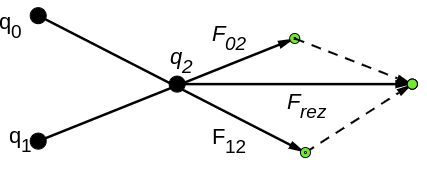
\includegraphics[scale=0.3]{superpoz.png}
\end{center}
\caption{\textit{Princip superpozicije}}
\label{fig:superpozicija}
\end{figure}

Kao sto je opisano u algoritmu \ref{alg:opsta_procedura}, u svakoj iteraciji se za svaku česticu računa njeno naelektrisanje imajući u vidu njenu vrednost ciljne funkcije. Jasno je da se naelektrisanje svake čestice menja u svakoj iteraciji.

Neka je sa $q^i$ označeno naelektrisanje čestice $x^i$. Tako dato naelektrisanje se računa po formuli: 
\begin{equation}
\label{eq:naelektrisanje}
q^i = exp\left(-n \cdot \frac{f(x^i) - f(x^{najbolje})}{\sum_{k=1}^{broj\_cestica} (f(x^k) - f(x^{najbolje})) }\right), i = \overline{1, broj\_cestica}    
\end{equation}
Iz jednacine \ref{eq:naelektrisanje} jasno sledi da će čestice koje imaju bolju vrednost ciljne funkcije imati veće naelektrisanje, i time više uticati na ostale čestice iz populacije, što je i bio jedan od zahteva opisan u poglavlju \ref{subsec:motivacija}. 

Kako se sav račun odvija u računaru, kod velikih populacija, razlomak može biti veoma mali pa može dovesti do prekoračenja ili potkoračenja pri izračunavanju eksponencijalne funkcije. Da bi se zaobišli takvi problemi, uvodi se množenje sa $n$\footnote{Dimenzija prostora dopustivih rešenja}. 

Naelektrisanje se računa u odnosu na ciljnu funkciju, postoje i alternativne metode, ali one neće biti opisane u ovom radu.

Kao što je navedeno u poglavlju \ref{subsec:motivacija}, postoje bitne razlike između elektromagnetizma u fizičkom smislu i onoga što se koristi u metaheuristikama. Naime, kako se može primetiti u formuli \ref{eq:naelektrisanje} nikakav znak se ne dodaje naelektrisanju $q^i$, što u fizici nije slučaj. Umesto davanja znakova naelektrisanjima, o smeru kretanja čestice se odlučuje drugačijom metodom - poređenjem ciljnih funkcija posmatrane i svake čestice koja deluje na nju. Tako se dobija $F^i$ koja predstavlja rezultujuću silu u čestici $i$:
\begin{equation}
    F^i = \sum_{j \neq i}^{broj\_cestica} 
    \begin{cases}
    $(x^j - x^i) \cdot \frac{q^i q^j}{\norm{x^j - x^i}^2}$, & \text{ako je $f(x^j) < f(x^i)$}. \\
    $(x^i - x^j) \cdot \frac{q^i q^j}{\norm{x^j - x^i}^2}$, & \text{ako je $f(x^j) \geq f(x^i)$}
    \end{cases}
\end{equation}

\begin{algorithm}[H]
\label{alg:izracunaj_sile}
\caption{$izracunaj\_sile()$}
\begin{algorithmic}[1]

\FOR{$i = 1$ \TO $broj\_cestica$}
\STATE $q^i \leftarrow exp\left(-n \frac{f(x^i) - f(x^{najbolje})}{\sum_{k=1}^{broj\_cestica}(f(x^k) - f(x^{najbolje})) }\right)$
\STATE $F^i \leftarrow 0$
\ENDFOR

\FOR{$i = 1$ \TO $broj\_cestica$}
\FOR{$j = 1$ \TO $broj\_cestica$}
\IF{$f(x^j) < f(x^i)$}
\STATE $F^i \leftarrow F^i + (x^j - x^i) \cdot \frac{q^i q^j}{\norm{x^j - x^i}^2} $ && \textit{privlačenje}
\ELSE
\STATE $F^i \leftarrow F^i - (x^j - x^i) \cdot \frac{q^i q^j}{\norm{x^j - x^i}^2} $ &&& \textit{odbijanje}
\ENDIF
\ENDFOR
\ENDFOR
\end{algorithmic}
\end{algorithm}

\subsubsection{Pomeranje čestica}
\label{subsec:pomeranje_cestice}
Nakon što sve čestice dobiju svoje naelektrisanje, i smer kretanja, potrebno ih je pomeriti kako bi se približili ka boljim rešenjima odnosno udaljili od loših. Za tu proceduru potrebno je izabrati parametar $\eta$ koji će predstavljati dužinu koraka. Ovde će biti izabran kao vrednost iz uniformne raspodele između 0 i 1, naravno da je moguće koristiti i neku drugu raspodelu, ali takvi slučajevi neće biti opisivani. Veličina koraka se u ovom slučaju uzima kao slučajan broj iz navedene raspodele kako bi postojala ne-nula verovatnoća kretanja ka neposećenim regionima.

\begin{equation}
\label{eq:pomeranje}
x^i = x^i + \eta \frac{F^i}{\norm{F^i}} V,i = \overline{1, broj\_cestica}
\end{equation}
Sa $V$ je dat vektor kretanja, čije komponente predstavljaju dozvoljena kretanja ka gornjoj granici $u_k$ i donjoj $l_k$. Normalizacija se vrši kako bi održali dopustivost rešenja.


\begin{algorithm}[H]
\label{alg:pomeri}
\caption{$pomeri()$}
\begin{algorithmic}[1]

\FOR{$i = 1$ \TO $broj\_cestica$}
\IF{$i \neq najbolje$}
\STATE $\eta \leftarrow \textit{U}[0, 1]$
\STATE $F^i \leftarrow \frac{F^i}{\norm{F^i}}$

\FOR{$k = 1$ \TO $n$}
\IF{$F^i_k > 0$}
\STATE $x_k^i \leftarrow x_k^i + \eta F^i_k (u_k - x_k^i)$
\ELSE
\STATE $x_k^i \leftarrow x_k^i + \eta F^i_k (x_k^i - l_k)$
\ENDIF
\ENDFOR
\ENDIF
\ENDFOR
\end{algorithmic}
\end{algorithm}

\section{UMAHLP problem}
\label{sec:umahlp}
Kako bi se razumeo kontekst problema, potrebno je prvo objasniti osnovne pojmove. Naime, u savremenim mrežama, kao što su telekomunikacione ili čak mreže pošte, moraju da postoje čvorovi koji odlučuju kome će sledećem poruka biti prosleđena kako bi došla do odredišta. Takvi čvorovi se nazivaju \textit{eng. hub}, i u daljem tekstu će se razlikovati od krajnjih čvorova koji učestvuju u komunikaciji.

\subsection{Formulacija problema}
\label{subsec:formulacija}
\textit{Uncapacitated multiple allocation hub location problem} je problem alokacije habova, odnosno izbora koji čvorovi u mreži treba da budu oni koji su zaduženi za rutiranje. Pritom nema ograničenja za broj čvorova koji mogu biti hubovi. Takođe, ne postavlja se ograničenje koliku količinu saobraćaja jedan hub može da prenese, niti jedan krajnji čvor mora pripadati samo jednom hubu. Uspostavljanje svakog huba zahteva određen trošak resursa. Cilj je rešiti problem tako da ukupna cena prenosa poruka i ukupan trošak za uspostavljanje hubova budu minimizovani.

Detaljnija objašnjenja problema i njegovih varijacija data su u radu \cite{formulation-UMAHLP}.
U nastavku biće data matematička formulacija problema. Korišćena je notacija iz literature \cite{UMAHLP}.

Pretpostavimo da je dato $n$ različitih čvorova u mreži. Neka je taj skup označen $S=\{1,..., n\}$, pritom svaki od čvorova može biti ili hub ili krajnji čvor. Neka je:
\begin{itemize}
    \item $C_{ij}$ rastojanje od i-tog do j-tog čvora
    \item $W_{ij}$ zahtev od i-tog do j-tog čvora
    \item $
    y_k=
    \begin{cases}
    $1$, & \text{ako je k-ti čvor hub}.\\
    $0$, & \text{inače}.
    \end{cases}
    $
    \item $x_{ijkm}$ predstavlja deo protoka $W_{ij}$ iz čvora $i$ koji je prikupljen od strane haba $k$, a prosleđen od strane haba $m$ do odredišnog čvora $j$
\end{itemize}
Kako se svaka putanja sastoji iz tri koraka:
\begin{enumerate}
    \item od početnog čvora do prvog haba
    \item transfer između habova
    \item prenos od poslednjeg haba do odredišnog čvora
\end{enumerate}
Uvode se parametri $\alpha$ koji predstavlja jediničnu cenu komunikacije hub-hub, i po definiciji je manji od 1. Parametri $\chi, \delta$ predstavljaju jedinične cene prikupljanja odnosno prenos do odredišnog čvora, redom. Tada je ciljna funkcija:
\begin{equation}
\label{eq:ciljna}
\min \sum_{i,j,k,m} W_{ij} \cdot (\chi \cdot C_{ik} + \alpha \cdot C_{km} + \delta \cdot C_{mj}) \cdot x_{ijkm} + \sum_{k} f_k \cdot y_k
\end{equation}
čiji ćemo minimum tražiti pri uslovima:
\begin{equation}
\label{ogr:2}
\sum_{k,m} x_{ijkm} = 1, \text{za sve i, j}
\end{equation}
\begin{equation}
\label{ogr:3}
\sum_{m} x_{ijkm} + \sum_{m,m\neq k}x_{ijmk} \leq y_k, \text{za sve i,j,k}
\end{equation}
\begin{equation}
\label{ogr:4}
y_k \in \{0, 1\}, \text{za svako k}
\end{equation}
\begin{equation}
\label{ogr:5}
x_{ijkm} \geq 0, \text{za sve i,j,k,m}
\end{equation}
Ograničenje \ref{ogr:2} govori da se svi protoci šalju između svih krajnjih čvorova, ograničenje \ref{ogr:3} garantuje da protok putuje samo preko otovorenih hubova. Ograničenja \ref{ogr:4} i \ref{ogr:5} garantuju ne-negativnost i binarnost promenljivih odlučivanja.

\subsection{Primena EM heuristike}
\label{subsec:primena}

Koristi se pristup već opisan u poglavlju \ref{subsec:procedura}. U nastavku će biti dat pseudokod i objašnjenja procedura koje su modifikovane.

\begin{algorithm}[H]
\label{alg:umahlp}
\caption{EM nad UMAHLP}
\begin{algorithmic}[1]
\STATE $inicijalizuj()$
\STATE $iter \leftarrow 1$
\WHILE{$iter < max\_iter$}

\FORALL{$x^k \text{u populaciji}$}
\STATE $izracunaj\_ciljnu()$
\STATE $1\_swap\_lokalna\_pretraga(x^k)$
\STATE $normalizuj(x^k)$
\ENDFOR
\STATE $izracunaj\_naelektrisanja\_i\_silu()$
\STATE $pomeri()$
\IF{$nema\_promena\_maksBrIteracija()$}
\STATE $kraj()$
\ENDIF
\STATE $iter \leftarrow iter + 1$
\ENDWHILE
\end{algorithmic}
\end{algorithm}
Kako je $y_k$ binarna promenljiva, njena vrednost se dobija po formuli:
\[ y_k = \begin{cases}
1,& \text{ako je } x_{k, i} \geq 0.5 \\
0,& \text{inače}
\end{cases}\]
Za svaki izabrani skup hubova, najkraći putevi do krajnjih čvorova u mreži se dobijaju Floyd-Warshallovim algoritmom (opisan u \cite{flojd-warsall}). Nakon nalaženja najkraćih puteva, između parova čvorova, vrši se evaluacija ciljne funkcije kako bi česticama bila dodeljena naelektrisanja i izračunati rezultujući vektori (sila kojom ostale čestice deluju na posmatranu i smer njenog kretanja). Sve procedure ostaju iste kao u poglavlju \ref{subsec:procedura}, osim lokalne pretrage. U ovoj heuristici se koristi tzv. \textit{1\_swap\_lokalna\_pretraga} i biće ukratko opisana.

Korišćena lokalna pretraga pokušava u svakoj iteraciji da zameni (\textit{eng. swap}) jedan element $y_k$ njenom komplementarnom vrednošću. Naime, ako je $y_k = 1$, dobija vrednost 0 i obrnuto. Što zapravo predstavlja da ako je čvor bio hub sada više nije. Proces lokalne pretrage se nastavlja kao što je opisano u poglavlju \ref{subsec:lokalna_pretraga}. Procedura normalizacije opisana je u poglavlju \ref{subsec:racunanje_sile}. 
Detaljniji opis rezultata metode i podacima nad kojim je primenjivana opisani su u radu \cite{UMAHLP} i prevazilaze okvire ovog teksta, te neće biti opisani.


\section{Izbor atributa}
\label{sec:izbor_atributa}
Izbor atributa (eng. \textit{feature selection}) je proces odabira podskupa atributa nekog skupa podataka. Izabrani podskup za cilj ima da najbolje, u poređenju sa ostalim podskupovima, ispunjava određeni kriterijum, npr. preciznost klasifikacije. Originalna formulacija problema i rešenja pomoću EM metaheuristike dati su u radu \cite{kartelj}.

Metode izbora atributa za cilj imaju smanjenje vremenskih i računskih troškova u rešavanju problema istraživanja podataka. Kako raste potreba za istraživanjem podataka, tako raste i njihova količina i dimenzionalnost. Samim tim, bitno je imati metod kojim se ti podaci mogu redukovati bez gubitka infomacija koje njihovi prvobitni atributi sadrže. U narednom poglavlju biće opisana heuristika bazirana na elektromagnetizmu primenjena na pomenuti problem.

\subsection{Opis algoritma}
\label{subsec:formulacija}
Sledeći parametri će biti korišćeni kao ulazni:
\begin{itemize}
    \item br\_iter - broj iteracija glavne petlje
    \item M - broj čestica
    \item $\alpha$ - skalirajući parametar iz [0, 1]
    \item r - instanca problema (skup podataka)
    \item N - dimenzija instance problema
\end{itemize}

Proces inicijalizacije čestica, detaljnije opisan u \ref{subsec:inicijalizacija}, se izvršava pozivanjem metode \textit{create random points} kojom se generiše vektor dimenzije M, dalje označen sa $p$. Svaka od koordinata jedne čestice je slučajno izabran broj iz intervala [0, 1].
Svaka od koordinata $i$-te čestice:
\begin{equation}
p_k^i=\begin{cases}
    $1$, & \text{ako je k-ti atribut uključen u rešenje}.\\
    $0$, & \text{inače}.
    \end{cases}, k=\overline{1, N}
\end{equation}

Kako se vrednosti biraju uniformno iz intervala [0, 1], koordinata se transformiše u binarnu po formuli:
\begin{equation}
\overline{p_k^i}=\begin{cases}
    $1$, & \text{ako je $p_k^i\geq0.5$} .\\
    $0$, & \text{inače}.
    \end{cases}, k=\overline{1, N}
\end{equation}
Vrednost praga 0.5 daje jednaku šansu svakom atributu ulaznog skupa da bude uključen ili ne.
Nakon inicijalizacije, u svakoj iteraciji glavne petlje se izračunava ciljna funkcija za svaku tačku. Postupak lokalne pretrage (poglavlje \ref{subsec:lokalna_pretraga}) se izvršava za tačku ako su ispunjeni uslovi: 
\begin{itemize}
    \item Tačka ima najbolji ili drugi najbolji rezultat
    \item Lokalna pretraga nije bila primenjivana na tu tačku ili joj se vrednost promenila u odnosu na poslednju loklanu pretragu.
    \item Najbolja vrednost se nije promenila u najmanje 10 poslednjih generacija
\end{itemize}
Kao algoritam lokalne pretrage, korišćena je metoda $1\_swap\_lokalna\_pretraga()$ opisana u poglavlju \ref{sec:umahlp}.

\subsection{Primena EM heuristike}
\label{subsec:primena}
Sama procedura algoritma se ne razlikuje od onog opisanog u poglavljima \ref{subsec:procedura} i \ref{sec:umahlp}. Kako je jedina razlika u izračunavanju ciljne funkcije, ona će biti opisana:
\begin{algorithm}[H]
\label{alg:elm}
\caption{ciljna\_funkcija($p_i, klasifikator$)}
\begin{algorithmic}[1]
\STATE $s_i = dekodiraj(p_i)$
\STATE $pronadjen \leftarrow pretrazi\_kes(p_i)$
\IF {$pronadjen == null$}
\IF {$klasifikator == 1NN$}
\STATE $obj \leftarrow 1nn\_5fold\_cv(s_i, r)$
\ELSE 
\STATE $obj \leftarrow svm\_2fold\_cv(s_i, r)$
\ENDIF
\STATE $dodaj\_u\_kes(s_i, obj)$
\ELSE 
\STATE $obj = dohvati\_iz\_kesa(s_i)$
\STATE $kesiraj(s_i)$
\ENDIF
\end{algorithmic}
\end{algorithm}
Kako bi se izbegla ponovljena izračunavanja nad istim podskupovima atributa, koristi se procedura keširanja, odnosno čuvanje rezultata računa u memoriji.

Metode $1nn\_5fold\_cv(s_i, r)$ i $svm\_2fold\_cv(s_i, r)$ klasifikuju dati ulazni skup podataka $r$ koristeći podskup skupa atributa $s_i$, i kao rezultat vraćaju preciznost klasifikatora. Izračunata preciznost predstavlja vrednost ciljne funkcije.

Naelektrisanje i rezultujuća sila svake čestice se računaju po postupku opisanom u poglavlju \ref{subsec:racunanje_sile}.

U slučajevima kada su vrednosti koordinata čestica bliske 0.5, dolazi do čestih promena koordinate iz 0 u 1 i obrnuto. Usled tih promena javlja se nepotrebno rasipanje pretrage i konvergencija algoritma opada.
Kako bi se ovo ponašanje izbeglo, standardni algoritam se modifikuje dodavanjem specijalne procedure skaliranja. Ako sa $p_k^i$ obeležimo $k$-tu koordinatu $i$-te čestice:
\begin{equation}
\label{eq:skala}
    p_k^i = \alpha \cdot s_k^i + (1 - \alpha) \cdot p_k^i
\end{equation}
Naime, uvedena procedura omogućava bolju kontrolu variranja vrednosti koordinata. Takođe, skaliranje ima svoje mane. Usled smanjenja prostora pretrage, može doći do prerane konvergencije, što dalje dovodi do dobijanja neoptimalnog rešenja. Nalaženje dobrog balansa između širenja i sužavanja prostora pretrage je ključno za ovakve metode.

Faktor skaliranja $\alfa$ uzima vrednosti iz skupa [0, 1]. U opštem slučaju, velike vrednosti ovog parametra dovode do lokalnog optimuma, a premale vrednosti neće ubrzati konvergenciju dovoljno. 

\subsection{Rezultati}
\label{sec:rezultati}

U narednoj tabeli \ref{tabela} prikazani su rezultati dobijeni u primenom elektromagnetne heuristike, i upoređeni su sa rezultatima dobijenim primenom metoda potpune pretrage, \textit{eng. Full Search} i genetskim algoritmom. \textit{Full Search} je metod pretrage po svim mogućim podskupovima skupa atributa. Rezultati preuzeti iz rada \cite{kartelj}.


\begin{table}[h]
\caption{Rezultati} \label{tabela}
\centering
\begin{center}
\small\addtolength{\tabcolsep}{-3pt}
\begin{tabular}{||c c c c c c C||}

\hline
skup podataka & br atributa & br klasa & br instanci & FS & genetski alg & EML \\ [0.1ex] 
\hline\hline
abalone & 8 & 11 & 3842 & 23.99 & 24.37 & opt \\ 
\hline
iris & 4 & 3 & 150 & 99.39 & 98.00 & opt \\
\hline
spambase & 57 & 2 & 4601 & - & 91.55 & 94.35\\
\hline
letter & 16 & 26 & 20000 & 96.39 & 95.24 & opt\\
\hline
\end{tabular}
\end{center}
\end{table}
Vrednost $opt$ opisuje slučaj kada je rezultat pri klasifikaciji, uz korišćenje metode za izbor atributa, bio identičan onome koji dobije metod potupne pretrage. 


\section{Zaključak}
\label{sec:zakljucak}

Elektromagnetna metaheuristika se može koristiti kao samostalan algoritam ili kao podrška nekim drugim algoritmima. Glavni koncept algoritma podrazumeva usmeravanja čestica prema lokalnim optimumima koristeći mehanizam privlačenja i odbijanja, i kao takav pokazuje dobre rezultate u praksi. Laka implementacija čini je pogodnom za rešavanje širokog skupa problema, uključujući i neke NP-teške.


% \section{Osnovna uputstva}
% Vaš seminarski rad mora da sadrži najmanje jednu \textbf{sliku}, najmanje jednu \textbf{tabelu} i najmanje \textbf{sedam referenci} u spisku literature. Najmanje jedna slika treba da bude originalna i da predstavlja neke podatke koje ste Vi osmislili da treba da prezentujete u svom radu. Isto važi i za najmanje jednu tabelu. 	Od referenci, neophodno je imati bar jednu \textbf{knjigu}, bar jedan \textbf{naučni članak} iz odgovarajućeg časopisa i bar jednu adekvatnu \textbf{veb adresu}. 

% \textbf{Dužina seminarskog rada treba da bude od 10 do 12 strana.} Svako prekoračenje ili potkoračenje biće kažnjeno sa odgovarajućim brojem poena. Eventualno, nakon strane 12, može se javiti samo tekst poglavlja \textbf{Dodatak} koji sadrži nekakav dodatni k\^{o}d, ali je svakako potrebno da rad može da se pročita i razume i bez čitanja tog dodatka. 

% Ко жели, може да пише рад ћирилицом. У том случају, неопходно је да су инсталирани одговарајући пакети: texlive-fonts-extra, texlive-latex-extra, texlive-lang-cyrillic, texlive-lang-other. 

% Nemojte koristiti stari način pisanja slova, tj ovo:
% \begin{verbatim}
% \v{s} i \v{c} i \'c ...
% \end{verbatim}
% Koristite direknto naša slova:	
% \begin{verbatim}
% š i č i ć ... 
% \end{verbatim}


% \section{Engleski termini i citiranje}	
% \label{sec:termini_i_citiranje}

% Na svakom mestu u tekstu naglasiti odakle tačno potiču informacije. Uz sve novouvedene termine u zagradi naglasiti od koje engleske reči termin potiče. 

% Naredni primeri ilustruju način uvođenja enlegskih termina kao i citiranje.

% \begin{primer}
% Problem zaustavljanja (eng.~{\em halting problem}) je neodlučiv \cite{haltingproblem}.
% \end{primer}

% \begin{primer}
% Za prevođenje programa napisanih u programskom jeziku C može se koristiti GCC kompajler \cite{gcc}.
% \end{primer}

% \begin{primer}
%  Da bi se ispitivala ispravost softvera, najpre je potrebno precizno definisati njegovo ponašanje \cite{laski2009software}. 
% \end{primer}

% Reference koje se koriste u ovom tekstu zadate su u datoteci {\em seminarski.bib}. Prevođenje u pdf format u Linux okruženju može se uraditi na sledeći način:
% \begin{verbatim}
% pdflatex TemaImePrezime.tex 
% bibtex TemaImePrezime.aux 
% pdflatex TemaImePrezime.tex 
% pdflatex TemaImePrezime.tex 
% \end{verbatim}
% Prvo latexovanje je neophodno da bi se generisao {\em .aux} fajl. {\em bibtex} proizvodi odgovarajući {\em .bbl} fajl koji se koristi za generisanje literature. 
% Potrebna su dva prolaza (dva puta pdflatex) da bi se reference ubacile u tekst (tj da ne bi ostali znakovi pitanja umesto referenci). Dodavanjem novih referenci potrebno je ponoviti ceo postupak.  











% Broj naslova i podnaslova je proizvoljan. Neophodni su samo Uvod i Zaključak. Na poglavlja unutar teksta referisati se po potrebi. 
% \begin{primer}
% U odeljku \ref{sec:naslov1} precizirani su osnovni pojmovi, dok su zaključci dati u odeljku \ref{sec:zakljucak}.
% \end{primer}

% Još jednom da napomenem da nema razloga da pišete:
% \begin{verbatim}
% \v{s} i \v{c} i \'c ...
% \end{verbatim}
% Možete koristiti srpska slova
% \begin{verbatim}
% š i č i ć ... 
% \end{verbatim}



% \section{Slike i tabele}
% \label{slike_i_tabele}

% Slike i tabele treba da budu u svom okruženju, sa odgovarajućim naslovima, obeležene labelom da koje omogućava referenciranje. 

% \begin{primer} Ovako se ubacuje slika. Obratiti pažnju da je dodato i 
% \begin{verbatim}
% \usepackage{graphicx}
% \end{verbatim}

% \begin{figure}[h!]
% \begin{center}
% \includegraphics[scale=0.75]{panda.jpg}
% \end{center}
% \caption{Pande}
% \label{fig:pande}
% \end{figure}

% Na svaku sliku neophodno je referisati se negde u tekstu. Na primer, na slici \ref{fig:pande} prikazane su pande. 
% \end{primer}

% \begin{primer} I tabele treba da budu u svom okruženju, i na njih je neophodno referisati se u tekstu. Na primer, u tabeli \ref{tab:tabela1} su prikazana različita poravnanja u tabelama.

% \begin{table}[h!]
% \begin{center}
% \caption{Razlčita poravnanja u okviru iste tabele ne treba koristiti jer su nepregledna.}
% \begin{tabular}{|c|l|r|} \hline
% centralno poravnanje& levo poravnanje& desno poravnanje\\ \hline
% a &b&c\\ \hline
% d &e&f\\ \hline
% \end{tabular}
% \label{tab:tabela1}
% \end{center}
% \end{table}

% \end{primer}

% \section{K\^{o}d i paket listings}
% Za ubacivanje koda koristite paket \textbf{listings}:
% \url{https://en.wikibooks.org/wiki/LaTeX/Source_Code_Listings}

% \begin{primer}
% Primer ubacivanja koda za programski jezik Python dat je kroz listing \ref{simple}. Za neki drugi programski jezik, treba podesiti odgvarajući programski jezik u okviru defnisanja stila.
% \end{primer}
% \begin{lstlisting}[caption={Primer ubacivanja koda u tekst},frame=single, label=simple]
% # This program adds up integers in the command line
% import sys
% try:
%     total = sum(int(arg) for arg in sys.argv[1:])
%     print 'sum =', total
% except ValueError:
%     print 'Please supply integer arguments'
% \end{lstlisting}


% \section{Prvi naslov}
% \label{sec:naslov1}


% Ovde pišem tekst. 
% Ovde pišem tekst. 
% Ovde pišem tekst. 
% Ovde pišem tekst. 
% Ovde pišem tekst. 
% Ovde pišem tekst. 
% Ovde pišem tekst. 
% Ovde pišem tekst. 


% \subsection{Prvi podnaslov}
% \label{subsec:podnaslov1}

% Ovde pišem tekst. 
% Ovde pišem tekst. 
% Ovde pišem tekst. 
% Ovde pišem tekst. 
% Ovde pišem tekst. 
% Ovde pišem tekst. 
% Ovde pišem tekst. 


% \section{Zaključak}
% \label{sec:zakljucak}

% Ovde pišem zaključak. 
% Ovde pišem zaključak. 
% Ovde pišem zaključak. 
% Ovde pišem zaključak. 
% Ovde pišem zaključak. 
% Ovde pišem zaključak. 
% Ovde pišem zaključak. 
% Ovde pišem zaključak. 
% Ovde pišem zaključak. 
% Ovde pišem zaključak. 
% Ovde pišem zaključak. 
% Ovde pišem zaključak. 


\addcontentsline{toc}{section}{Literatura}
\appendix
\bibliography{seminarski} 
\bibliographystyle{plain}

% \appendix
% \section{Dodatak}
% Ovde pišem dodatne stvari, ukoliko za time ima potrebe.
% Ovde pišem dodatne stvari, ukoliko za time ima potrebe.
% Ovde pišem dodatne stvari, ukoliko za time ima potrebe.
% Ovde pišem dodatne stvari, ukoliko za time ima potrebe.
% Ovde pišem dodatne stvari, ukoliko za time ima potrebe.


\end{document}
